
 \LabHeader{6}{1}

%{\large
\begin{enumerate}
\item \textbf{Шахова тура.} Розташування тури на шахівниці задано парою чисел $(i, j)$, $1\leqslant i, j\leqslant 8$. Вивести схематично шахову дошку, позначаючи символом \mintinline{python}{'+'} ті поля, куди <<б'є>> тура, і символом \mintinline{python}{'-'} "--- всі інші поля.

{\itshape Тура <<б'є>> по горизонталі та вертикалі.}

\item \textbf{Послідовність.} Послідовність $\{a_n\}$ задана рекурентно:
\begin{gather*}
a_1=1, \quad a_2=2, \quad a_3=3, \\
a_k = a_{k-1}+a_{k-2}-2\, a_{k-3}, \; k\geqslant 4.
\end{gather*}

Дано натуральне число $n$. Знайти максимальний серед елементів $a_1$, $a_2$, \ldots, $a_n$, а також його номер у пос\-лі\-дов\-нос\-ті.
\end{enumerate}
%}

 

 \LabHeader{6}{2}

%{\large
\begin{enumerate}
\item \textbf{Трикутні числа.} {\itshape Трикутним числом}\footnote[1]{Назви чисел, пов'язані з геометричними фігурами, сягають піфагорійців.} називається число кругів, які можуть бути розставлені у формі правильного три\-кут\-ни\-ка (див. малюнок).
\begin{center}
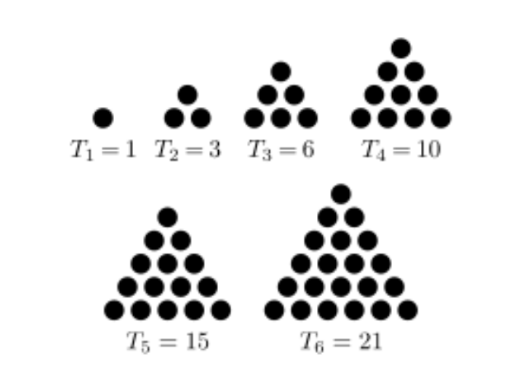
\includegraphics[width=0.55\textwidth]{trnum.png}
\end{center}

Дано натуральне число $n$.
Вивести на екран трикутні числа $T_1$, $T_2$, \ldots, $T_n$.

{\itshape * Що являє собою сума двох сусідніх трикутних чисел? Спробуйте здогадатися, чому.}
\item \textbf{Шахова дошка.} Вивести на екран схематичне зображення шахової дошки, позначаючи нулями білі поля, одиницями "--- чорні.
{\itshape Праве нижнє поле дошки завжди білого кольору.}
\end{enumerate}
%}

 

 \LabHeader{6}{3}

%{\large
\begin{enumerate}
\item \textbf{Таблиця.} Дано натуральне число $n$. Надрукувати таб\-ли\-цю такого вигляду:
{\ttfamily
\begin{center}
\setlength{\tabcolsep}{6pt}
\begin{tabular}{ccccc}
0 & 1 & 2 & $\ldots$ & n \\
1 & 2 & 3 & $\ldots$ & n+1 \\
2 & 3 & 4 & $\ldots$ & n+2 \\
$\cdots$ & $\cdots$ & $\cdots$ & $\ddots$ & $\cdots$ \\
n & n+1 & n+2 & $\ldots$ & 2n
\end{tabular}
\end{center}
}
\item \textbf{Квадрати.} Відома наступна закономірність:
$$
\begin{array}{lcl}
1^2 & = & 1\\
2^2 & = & 1+3\\
3^2 & = & 1+3+5\\
4^2 & = & 1+3+5+7\\
\ldots &
\end{array}
$$

Дано натуральне число $n$. Знайти квадрат, використовуючи цю закономірність.

{\itshape *Спробуйте довести цю формулу з геометричних міркувань.}
\end{enumerate}
%}

 

 \LabHeader{6}{4}

%{\large
\begin{enumerate}
\item \textbf{Автоморфні числа.} Натуральне число називається {\itshape автоморфним}, якщо десятковий запис його квадрата закінчується цифрами самого числа. Наприклад, числа 5, 76, 2\,890\,625 є автоморфними:
$$
\mathbf{5}^2=2\mathbf{5}; \quad \mathbf{76}^2=57\mathbf{76}; \quad \mathbf{2890625}^2=835571\mathbf{2890625}.
$$

Знайти та вивести на екран усі трицифрові автоморфні числа.
\item \textbf{Таблиця.} Дано натуральне число $n$. Надрукувати таблицю розміром \\$(2n+1)\times n$ такого вигляду:
{\ttfamily
\begin{center}
\setlength{\tabcolsep}{6pt}
\begin{tabular}{cccccc}
1 & 2 & 3 & $\ldots$ & n-1 & n \\
n & n-1 & n-2 & $\ldots$ & 2 & 1 \\
1 & 2 & 3 & $\ldots$ & n-1 & n  \\
$\cdots$ & $\cdots$ & $\cdots$ & $\ddots$ & $\cdots$ & $\cdots$ \\
n & n-1 & n-2 & $\ldots$ & 2 & 1 \\
1 & 2 & 3 & $\ldots$ & n-1 & n
\end{tabular}
\end{center}
}
\end{enumerate}
%}

 

 \LabHeader{6}{5}

%{\large
\begin{enumerate}
\item \textbf{Таблиця.} Дано натуральне число $n\geqslant 3$. Надрукувати таблицю розміром $10\times n$ такого вигляду:
{\ttfamily
\begin{center}
\setlength{\tabcolsep}{6pt}
\begin{tabular}{ccccc}
1 & 2 & 3 & $\ldots$ & n \\
1 & 2 & 3 & $\ldots$ & n \\
1 & 2 & 3 & $\ldots$ & n \\
$\cdots$ & $\cdots$ & $\cdots$ & $\ddots$ & $\cdots$ \\
1 & 2 & 3 & $\ldots$ & n
\end{tabular}
\end{center}
}
\item \textbf{Депозит.} Ерік Айдл відкрив рахунок у банку, вклавши 1000 фунтів стерлінгів. Згідно з умовами вкладу, сума на рахунку збільшується на 2 відсотки щомісяця. Вивести суму на рахунку містера Айдла через три, чотири, дванадцять місяців. На скільки відсотків зросте його внесок протягом року?
\end{enumerate}
%}

 

 \LabHeader{6}{6}

%{\large
\begin{enumerate}
\item \textbf{Послідовність.} Послідовність $\{a_n\}$ задана рекурентно:
\begin{gather*}
a_1=1,\quad a_2=2,\quad a_3=3,\\
a_k = a_{k-1}+a_{k-2}-2a_{k-3}, \; k\geqslant 4.
\end{gather*}

Дано натуральне число $n$. Знайти мінімальний серед елементів $a_1$, $a_2$, \ldots, $a_n$, а також його номер у пос\-лі\-до\-вно\-сті.
%\item {\bfseries Гра <<Вгадай число 2.0>>.} Комп'ютер <<загадує>> випадкове ціле число від 0 до 9. Гравцю надається три спроби вгадати це число. У ході «діалогу» ком-п'ютер дає підказки («більше», «менше»). У разі успіху гравцеві видається повідомлення про виграш, а після третьої невдалої спроби -- про програш.
\item \textbf{Таблиця.} Дано натуральне число $n\geqslant 3$. Надрукувати таблицю розміром $n\times 11$ такого вигляду:
{\ttfamily
\begin{center}
\setlength{\tabcolsep}{6pt}
\begin{tabular}{ccccc}
10 & 11 & 12 & $\ldots$ & 20 \\
20 & 21 & 22 & $\ldots$ & 30 \\
30 & 31 & 32 & $\ldots$ & 40  \\
$\cdots$ & $\cdots$ & $\cdots$ & $\ddots$ & $\cdots$ \\
\end{tabular}
\end{center}
}
\end{enumerate}
%}

 

 \LabHeader{6}{7}

%{\large
\begin{enumerate}
\item \textbf{Тренування.} Почавши тренування, спортсмен у перший день пробіг 10 км. Кожен наступний день він збільшував пробіг на 10%. Визначити:
\begin{itemize}[noitemsep, label=\faForward]
\item скільки пробіг спортсмен за другий, третій, \ldots, десятий день тренувань;
\item сумарний шлях, який пробіг спортсмен за перший тиждень тренувань.
\end{itemize}
\item \textbf{Таблиця.} Дано натуральне число $n$. Надрукувати таблицю розміром $n\times n$ такого вигляду:
{\ttfamily
\begin{center}
\setlength{\tabcolsep}{6pt}
\begin{tabular}{cccccc}
1 & 1 & 1 & $\ldots$ & 1 & 1 \\
1 & 0 & 0 & $\ldots$ & 0 & 1 \\
1 & 0 & 0 & $\ldots$ & 0 & 1  \\
$\cdots$ & $\cdots$ & $\cdots$ & $\ddots$ & $\cdots$ & $\cdots$\\
1 & 0 & 0 & $\ldots$ & 0 & 1 \\
1 & 1 & 1 & $\ldots$ & 1 & 1
\end{tabular}
\end{center}
}
\end{enumerate}
%}

 

 \LabHeader{6}{8}

%{\large
\begin{enumerate}
\item \textbf{Тренування.} Почавши тренування, спортсмен у перший день пробіг 5 км. Кожен наступний день він збільшував пробіг на 20%. Визначити:
\begin{itemize}[noitemsep, label=\faForward]
\item скільки пробіг спортсмен за другий, третій, \ldots, десятий день тренувань;
\item сумарний шлях, який пробіг спортсмен за десять днів тренувань.
\end{itemize}
\item
%\begin{multicols}{2}
\textbf{Таблиця множення.} Дано натуральне число $n$. Вивести стовпець таблиці множення, відповідний цьому числу.

Наприклад, при $n=5$ результат повинен мати такий вигляд:\\
%\includegraphics{table.png}
%\end{multicols}
\begin{results}
Enter a number, please: 5\\
5 x 1 = 5\\
5 x 2 = 10\\
5 x 3 = 15\\
5 x 4 = 20\\
5 x 5 = 25\\
5 x 6 = 30\\
5 x 7 = 35\\
5 x 8 = 40\\
5 x 9 = 45\\
\end{results}
\end{enumerate}
%}

 

 \LabHeader{6}{9}

%{\large
\begin{enumerate}
\item \textbf{Цукерки.} Відома ціна 1 кг цукерок <<Spam!>>. Вивести на екран таблицю вартості 100, 200, 300, \ldots, 1000 г цих цукерок.

\item \textbf{Таблиця.} Дано натуральне число $n$. Надрукувати таблицю розміром $n\times n$ такого вигляду:
{\ttfamily
	\begin{center}
		\setlength{\tabcolsep}{6pt}
		\begin{tabular}{cccccc}
			1 & 2 & 3 & $\ldots$ & n-1 & n \\
			1 & 2 & 0 & $\ldots$ & 0 & n \\
			1 & 0 & 3 & $\ldots$ & 0 & n  \\
			$\cdots$ & $\cdots$ & $\cdots$ & $\ddots$ & $\cdots$ & $\cdots$\\
			1 & 0 & 0 & $\ldots$ & n-1 & n \\
			1 & 2 & 3 & $\ldots$ & n-1 & n
		\end{tabular}
	\end{center}
}
%\includegraphics{table.png}
%\end{multicols}
%\begin{center}
%\includegraphics{table.png}
%\end{center}
\end{enumerate}
%}

 

 \LabHeader{6}{10}

%{\large
\begin{enumerate}
\item \textbf{Хід ферзем.} Розташування ферзя на шахівниці задано парою чисел $(i, j)$, $1\leqslant i, j\leqslant 8$. Вивести схематично шахівницю, позначаючи символом \mintinline{python}{'+'} ті поля, куди <<б'є>> ферзь, і символом \mintinline{python}{'-'} "--- всі інші поля.
%\item Послідовність {\itshape чисел Фібоначчі} задається наступним чином:
%$$
%F_1=F_2=1,\quad F_{n}=F_{n-1}+F_{n-2}, \; n \ geqslant 3.
%$$
%Перевірити справедливість тотожності
%$$
%F_1+F_3+F_5+\ldots+F_{2n-1}=F_{2n}
%$$
%для перших 20 значень $n$.
\item \textbf{Піфагорові трійки.} Дано натуральне число $k\leqslant 50$. Вивести всі піфагорові трійки чисел $(a, b, c)$, де $a<b<c$ і~$c\leqslant k$.

{\itshape Числа $a$, $b$, $c$ утворюють піфагорову трійку, якщо $$c^2=a^2+b^2.$$}
\end{enumerate}
%}

 

 \LabHeader{6}{11}

%{\large
\begin{enumerate}
\item {\bfseries Гра <<Вгадай число 1.0>>.} Комп'ютер <<загадує>> випадкове ціле число від 0 до 9. Гравцю  надається три спроби вгадати це число. У ході «діалогу» комп'ютер дає підказки («більше», «менше»). У разі успіху гравцеві видається повідомлення про виграш, а після третьої невдалої спроби -- про програш.
\item \textbf{Таблиця.} Дано натуральне число $n$. Надрукувати таблицю роз\-мі\-ром $n\times n$ такого вигляду:
{\ttfamily
\begin{center}
\setlength{\tabcolsep}{6pt}
\begin{tabular}{ccccc}
1 & 0 & 0 & $\ldots$ & 0 \\
0 & 1 & 0 & $\ldots$ & 0 \\
0 & 0 & 1 & $\ldots$ & 0 \\
$\cdots$ & $\cdots$ & $\cdots$ & $\ddots$ & $\cdots$ \\
0 & 0 & 0 & $\ldots$ & 1
\end{tabular}
\end{center}
}
\end{enumerate}
%}

 

 \LabHeader{6}{12}

%{\large
\begin{enumerate}
\item \textbf{Таблиця додавання.} Дано натуральне число $q\leqslant 10$. Надрукувати таблицю додавання для $q$-їчної системи числення.
\item \textbf{Квадрати Фібоначчі.} Послідовність {\itshape чисел Фібоначчі} задається такою формулою:
$$
F_1=F_2=1,\quad F_{n}=F_{n-1}+F_{n-2}, \; n \geqslant 3.
$$
Перевірити справедливість тотожності\footnote[1]{Ця формула має гарне геометричне доведення. {\itshape Яке?}}
$$
F_1^2+F_2^2+\ldots+F_n^2=F_{n}\cdot F_{n+1}
$$
для перших 20 значень $n$.


\end{enumerate}
%}

 

 \LabHeader{6}{13}

%{\large
\begin{enumerate}
\item \textbf{Сума факторіалів.} {\itshape Факторіалом}\ натурального числа $n$ називається добуток всіх натуральних чисел від 1 до $n$ включно:
$$
n! = 1 \cdot 2 \cdot 3 \cdot \ldots \cdot n.
$$

Дано натуральне число $k$. Знайти суму факторіалів перших $k$ натуральних чисел.
\item \textbf{Таблиця.} Дано натуральне число $n$. Надрукувати таблицю роз\-мі\-ром $n\times n$ такого вигляду:
{\ttfamily
\begin{center}
\setlength{\tabcolsep}{6pt}
\begin{tabular}{ccccccc}
0 & 0 & 0 & $\ldots$ & 0 & 0 & 1 \\
0 & 0 & 0 & $\ldots$ & 0 & 1 & \\
0 & 0 & 0 & $\ldots$ & 1 &  \\
$\cdots$ & $\cdots$ & $\cdots$ & $\ldots$ &  \\
0 & 0 & 1 & \\
0 & 1 & \\
1 &
\end{tabular}
\end{center}
}
\end{enumerate}
%}

 

 \LabHeader{6}{14}

%{\large
\begin{enumerate}
\item \textbf{Таблиця.} Дано натуральне число $n$. Надрукувати таблицю такого вигляду:
{\ttfamily
\begin{center}
\setlength{\tabcolsep}{6pt}
\begin{tabular}{ccccc}
1 & \\%0 & 0 & $\ldots$ & 0 \\
0 & 2 & \\%0 & $\ldots$ & 0 \\
0 & 0 & 3 & \\%\ldots & 0 \\
$\cdots$ & $\cdots$ & $\cdots$ & $\ddots$ & \\%$\cdots$ \\
0 & 0 & 0 & $\ldots$ & n
\end{tabular}
\end{center}
}
\item {\bfseries Гра <<Вгадай число 1.0>>.} Комп'ютер <<загадує>> випадкове ціле число від 0 до 9. Гравцю  надається три спроби вгадати це число. У ході «діалогу» ком-п'ютер дає підказки («більше», «менше»). У разі успіху гравцеві видається повідомлення про виграш, а після третьої невдалої спроби -- про програш.
\end{enumerate}
%}

 

 \LabHeader{6}{15}

%{\large
\begin{enumerate}
\item \textbf{Дружні числа.} Два натуральні числа називаються {\itshape дружніми}, якщо кожне з них дорівнює сумі дільників іншого (не враховуючи саме число). Такі, наприклад, числа 220 і 284 (вони були відомі ще піфагорійцям \footnote [1] {Сума дільників числа 220 дорівнює 1 +2 +4 +5 +10 +11 +20 +22 +44 +55 +110 = 284; сума дільників числа 284 дорівнює 1+2+4+71+142=220.}).

Вивести на екран усі пари дружніх чисел, що не перевищують 10,000.
\item \textbf{Таблиця.} Дано непарне натуральне число $n\geqslant 3$. Надрукувати таблицю розміром $n\times n$ такого вигляду:
{\ttfamily
\begin{center}
\setlength{\tabcolsep}{6pt}
\begin{tabular}{ccccc}
n & n & n & $\ldots$ & n \\
0 & 0 & 0 & $\ldots$ & 0 \\
n & n & n & $\ldots$ & n  \\
$\cdots$ & $\cdots$ & $\cdots$ & $\ddots$ & $\cdots$ \\
0 & 0 & 0 & $\ldots$ & 0 \\
n & n & n & $\ldots$ & n 
\end{tabular}
\end{center}
}
\end{enumerate}

